% Two paths alpha (upper, curved) and beta (lower, straight) with the same
% endpoints inside a simply connected region Omega.
% Source: book/tex/complex-ana/holomorphic.tex (section: Cauchy-Goursat theorem).
\documentclass[border=2mm]{standalone}
\usepackage{tikz}
\usetikzlibrary{arrows.meta}
\begin{document}
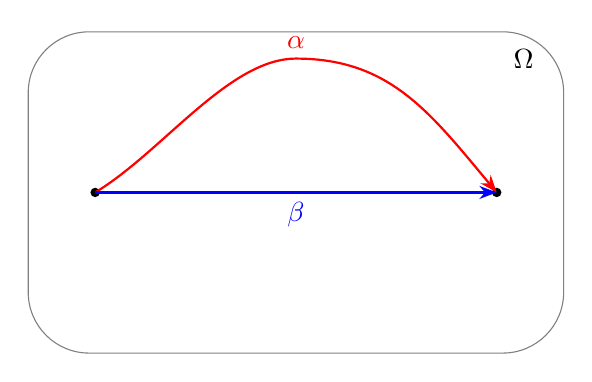
\begin{tikzpicture}[scale=0.85, >={Stealth[length=2.2mm]}]
  \draw[rounded corners=22pt, gray] (-4,-2.4) rectangle (4,2.4);
  \node at (3.4,2) {$\Omega$};
  \fill (-3,0) circle (2pt);
  \fill (3,0) circle (2pt);
  \draw[red, thick, ->] (-3,0) .. controls (-2,0.6) and (-1,2) .. (0,2)
                                .. controls (1.4,2) and (2,1.2) .. (3,0);
  \node[red, above] at (0,2) {$\alpha$};
  \draw[blue, thick, ->] (-3,0) -- (3,0);
  \node[blue, below] at (0,0) {$\beta$};
\end{tikzpicture}
\end{document}
